%!TEX root = ../main.tex
%******************************
%	 Chapter 1 
%*****************************

\chapter{Ageing increases transcriptional noise in CD4$^+$ T cell activation}

\graphicspath{{"../../Dropbox (Cambridge  University)/Figures_for_thesis/Chapter1/"}}

\vfill

\begin{Abstract}
Ageing is characterised by progressive loss of physiological and cellular functions, but the molecular basis of this decline remains largely unexplored. Here, we explored how ageing impacts transcriptional dynamics using single-cell RNA-sequencing of over a thousand unstimulated and stimulated naive and effector memory CD4$^+$ T cells from young and old mice. Furthermore, we sampled cells from two divergent strains of mice to assess the evolutionary conservation of the molecular ageing signature. In young animals, immunological activation drives a transcriptomic switch from variable to tightly regulated gene expression, characterised by a strong up-regulation of a core activation program, coupled with a decrease in cell-to-cell variability. The up-regulation of a set of immune response genes is conserved between the two mouse strains as is the decrease in expression variability upon immune activation. Ageing significantly perturbed the activation of the core immune response program by increasing expression heterogeneity across different populations of CD4$^+$ T cells. This discovery adds transcriptional noise as an unexplored hallmark of ageing to the list of known phenotypic changes.
\end{Abstract}

\vfill

\newpage

\begin{Comment}
\textbf{Declaration} This work was a joint effort of the Marioni, Odom, de la Roche and Teichmann labs. Celia P. Martinez-Jimenez, Duncan T. Odom, John C. Marioni and Sarah Teichmann designed the study. Celia P. Martinez-Jimenez and Aleksandra A. Kolodziejczyk performed preliminary experiments. Celia P. Martinez-Jimenez performed all single-cell RNA sequencing experiments displayed in this chapter. Hung-Chang Chen and Maike de la Roche provided extensive support during the revision process. Hung-Chang Chen performed FACS experiments during the revision process. Lovorka Stojic and Frances Connor provided experimental support. Timothy F. Rayner provided technical support. Michael J. T. Stubbington performed the T cell receptor and clone analysis. Catalina A. Vallejos helped with the statistical analysis by providing additional explanations of the BASiCS model. Celia P. Martinez-Jimenez and I interpreted results. Celia P. Martinez-Jimenez, Duncan T. Odom, John C. Marioni and I wrote the manuscript. Duncan T. Odom and John C. Marioni supervised the study. I performed computational analysis of all data displayed in this chapter and generated all figures with the exception of the FACS analysis (Fig. \ref{fig1:FACS} and Fig. \ref{fig1:EM_Naive_CD4}A-C). The paper has been published as:\\

Celia P. Martinez-Jimenez$^\ast$, Nils  Eling$^\ast$, Hung-Chang Chen, Catalina A. Vallejos, Aleksandra Kolodziejczyk, Frances Connor, Lovorka Stojic, Tim F. Rayner, Michael J. T. Stubbington, Sarah A. Teichmann, Maike de la Roche, John C. Marioni, Duncan T. Odom. Ageing increases cell-to-cell transcriptional variability upon immune stimulation. \emph{Science}, 1436: 1433-1436, 2017, ($^\ast$ equal contributions)
\end{Comment}

\begin{figure}[hb]
\centering    
\includegraphics[width=0.8\textwidth]{GraphicalAbstract.png}
\end{figure}

\newpage

% Include different main sections of the first chapter
%!TEX root = ../chapter1.tex
%******************************
%	 Introduction 
%*****************************

\section{Introduction} 

Ageing is characterized by the progressive decline of physiological and cellular functions \citep{Lopez-Otin2013, Booth2016}. It can have a complex and tissue-specific impact on gene expression levels \citep{Zahn2007}, as seen by microarray expression analyses of collections of mouse CD4$^+$ and CD8$^+$ T cells \citep{Mirza2011}, rat hepatocytes \citep{Tollet-Egnell2000}, mouse and human brain \citep{Lu2004, Lee2000}, human muscle \citep{Welle2003, Zahn2006}, human kidney \citep{Rodwell2004}, human retina \citep{Yoshida2002}, and different species of Drosophila and Caenorhabditis \citep{Mccarroll2004}. For instance, aging affects distinct functional pathways, even in closely related CD4$^+$ and CD8$^+$ T cells \citep{Mirza2011}. \\

Approaches that analyse the expression of sets of genes on a single-cell basis have more recently suggested that ageing may also alter the cell-to-cell variability of gene expression. Analysis of fifteen genes in terminally differentiated cardiomyocytes suggested that aging can lead to increased cell-to-cell transcriptional variability \citep{Bahar2006}. In contrast, single-cell analysis of the transcription of six genes in four different hematopoietic stem cell types showed few cell-to-cell changes between old and young animals, leading to the suggestion that transcriptional instability may not be a universal attribute of ageing \citep{Warren2007}. Whether cell-to-cell gene expression variability increases during ageing on a genome-wide basis, particularly for dynamic activation programs, remains largely unexplored.\\

Single-cell RNA sequencing can now allow the quantification of transcriptional variability in thousands of genes simultaneously. For example, Kowalczyk \textit{et al.} performed a high-resolution scRNA-seq analysis of hematopoietic stem cells in young and old mice. Here, cell cycle is the primary driver for cell-to-cell variability in gene expression, and aging decreases the entry of long-term hematopoietic stem cells into G1 phase in a cell-type-specific manner \citep{Kowalczyk2015}.\\ 

Naive CD4$^+$ T cells are an excellent model system to evaluate the impact of ageing on gene expression levels and cell-to-cell transcriptional variability. They are readily isolated as single, phenotypically homogeneous cells when purified from young and aged spleens and can be easily stimulated into a physiologically-relevant activated transcriptional state in vitro. Naive CD4$^+$ T cells are maintained in a quiescent state, but have the ability to respond to antigen stimulation with proliferation and effector differentiation, which is essential for life-long maintenance of adaptive immune function against infection and cancer \citep{Swain2012, Kim2014a}. \\

A conserved set of response genes has been identified by comparison of bulk gene expression between human and mouse CD4$^+$ T cells after immune activation \citep{Shay2013}. Indeed, as a strategy, comparison of gene expression levels in matched tissues from different mammalian species is a powerful tool for revealing conserved cell-type-specific regulatory programs \citep{Sudmant2015, Finseth2014, Brawand2011, Flajnik2009}. It is not known whether conservation of gene expression levels is also reflected in cell-to-cell variability.\\

Here, we dissect the activation dynamics of naive CD4$^+$ T cells at the single cell level during ageing in two sub-species of mice. In young and old animals, immune activation causes the up-regulation of hundreds of target genes, coupled to a strong decrease in cell-to-cell transcriptional variability across all genes. Ageing had only modest and species-specific effects on gene expression levels, but substantially increased cell-to-cell transcriptional variability in naive cells and effector memory cells upon activation.

\newpage
%!TEX root = ../chapter1.tex
%******************************
%	 Results 
%*****************************

\section{scRNAseq of murine CD4$^+$ T cells}
\subsection*{Single-cell RNA sequencing of CD4$^+$ T cells during activation, ageing and across two mouse species}

\begin{wrapfigure}{r}{0.5\textwidth}
\centering    
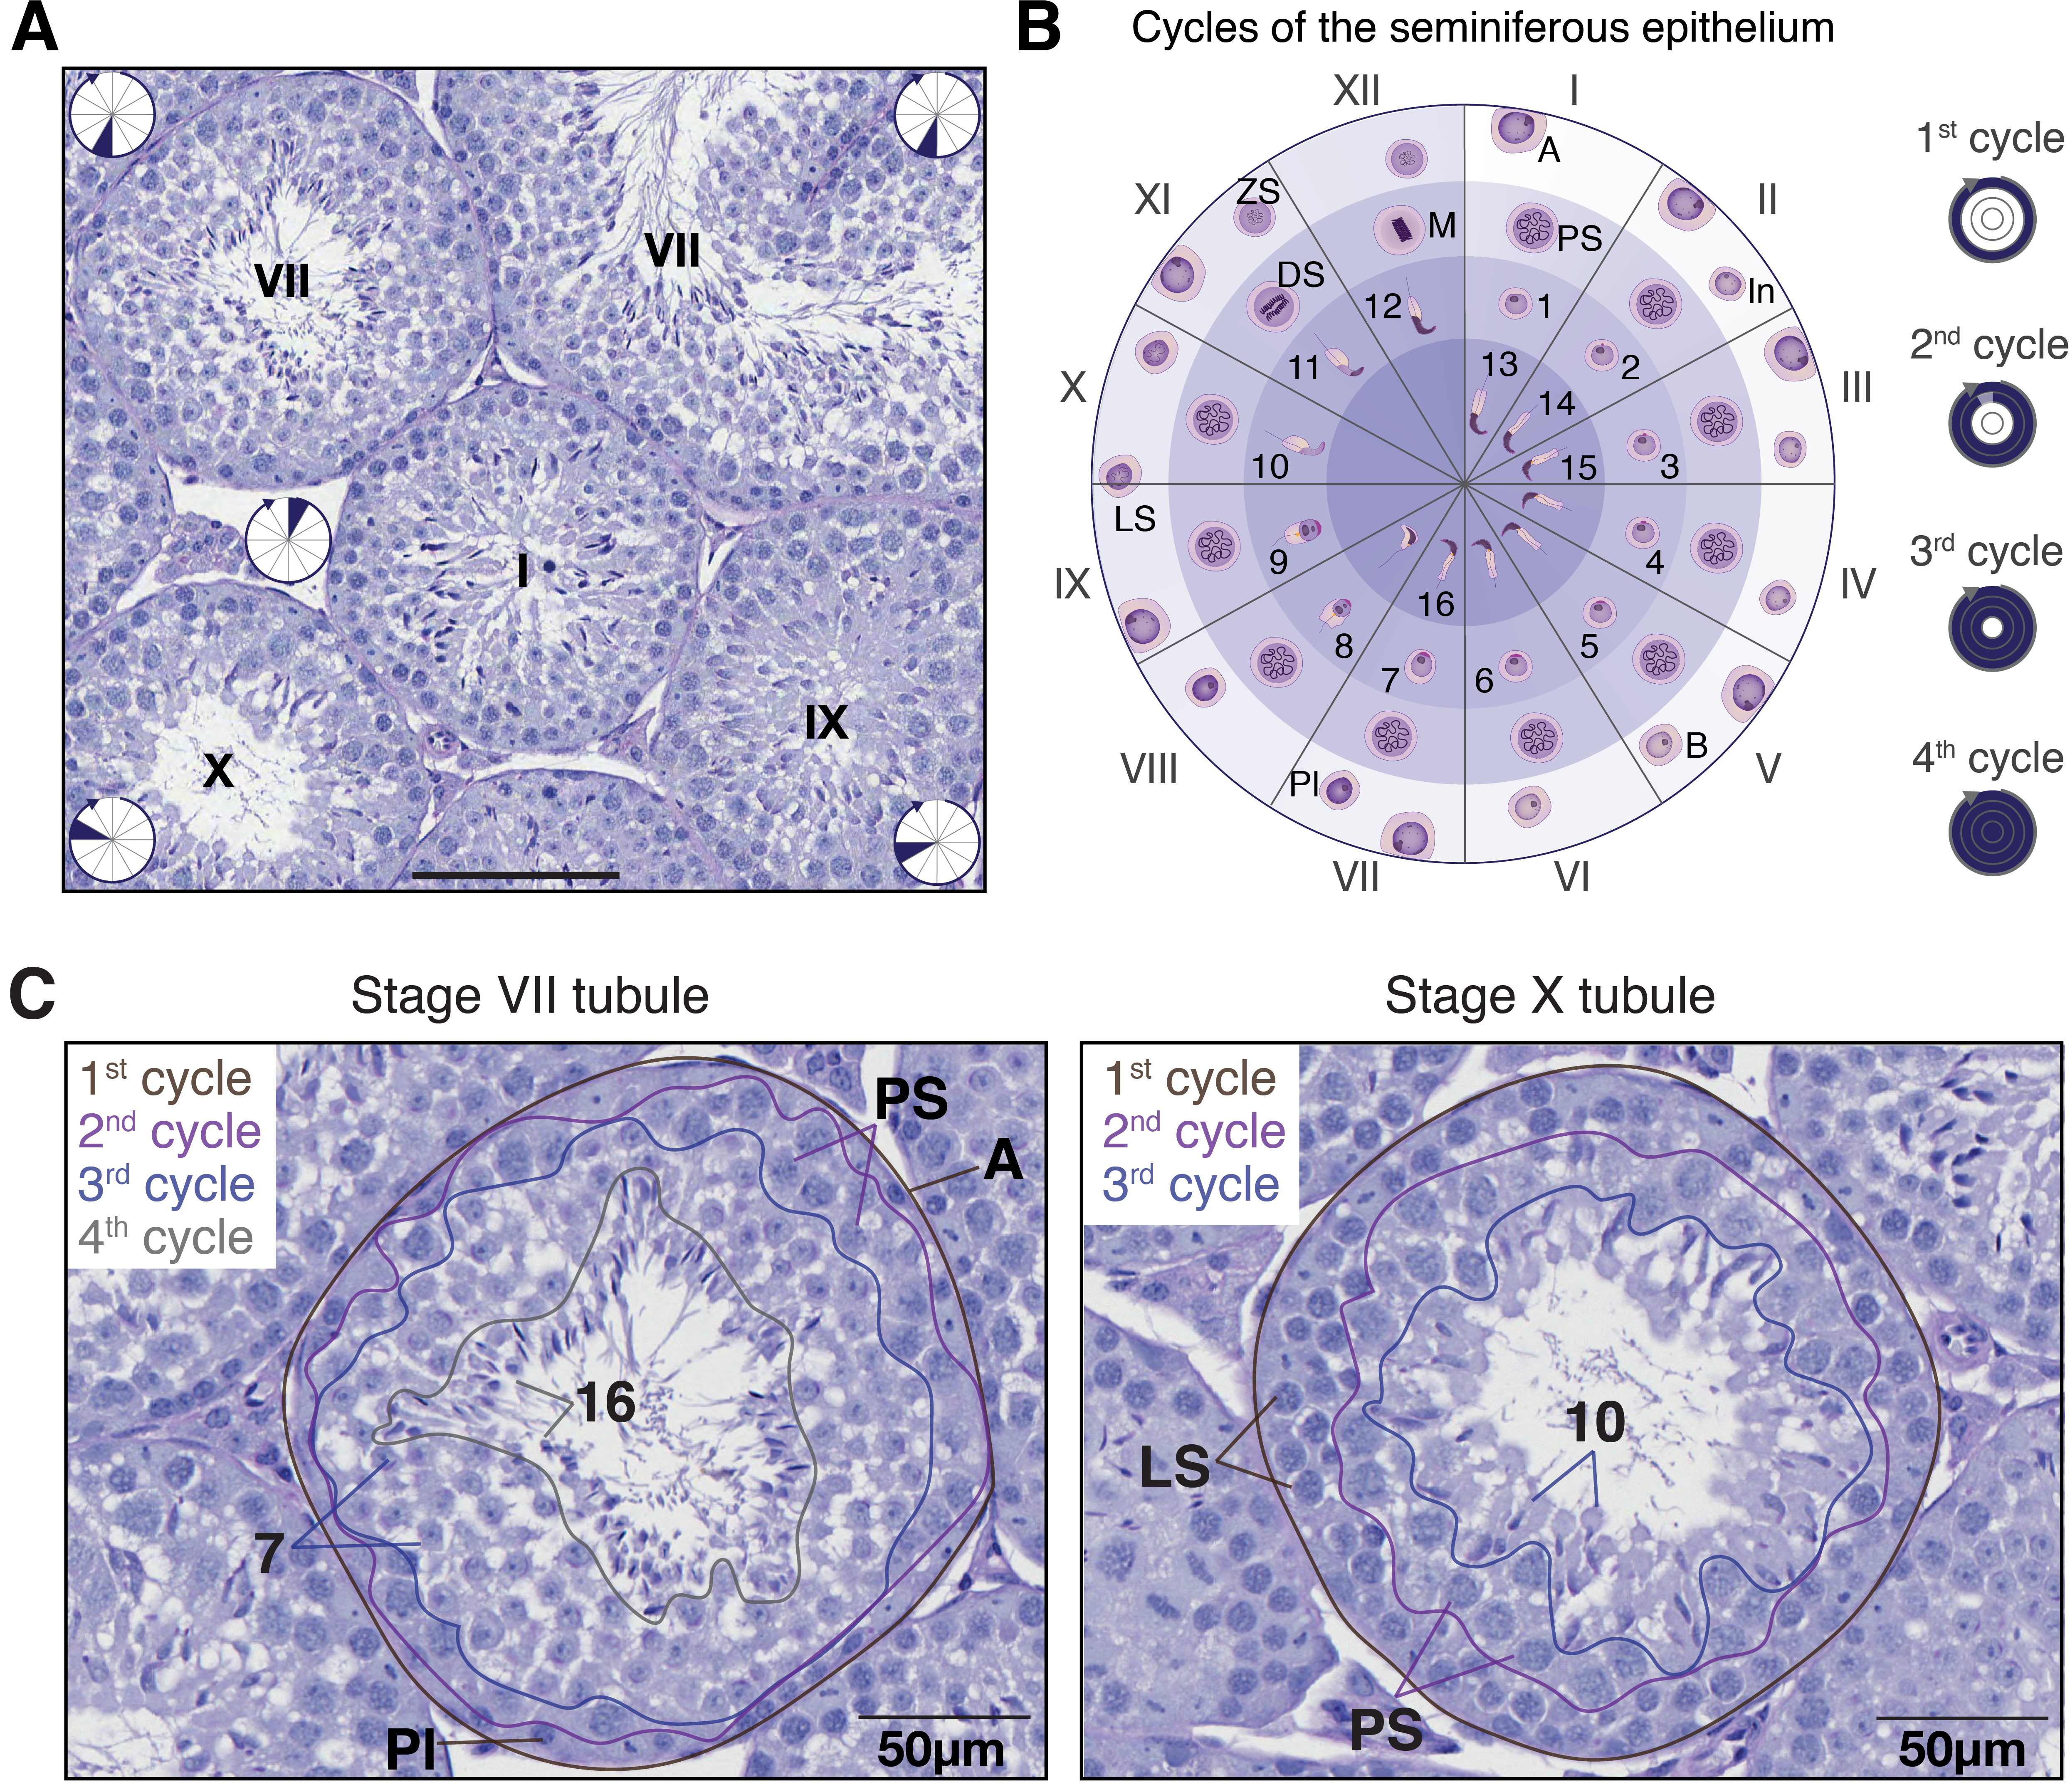
\includegraphics[width=0.48\textwidth]{Fig_1.png}
\caption[scRNAseq of CD4$^+$ T cells from young and old mice.]{\textbf{scRNAseq of unstimulated and activated CD4$^+$ T cells from young and old B6 and CAST animals.} \\
Single cells were isolated from spleens of young (~3 month) and old (~21 month) individuals of two related mouse sub-species (Mus musculus domesticus, B6; Mus musculus castaneus, CAST). Isolated cells were subjected to single-cell mRNA sequencing (scRNAseq) before or after 3 hours of in vitro activation using anti-CD3$\epsilon$/CD28 coated plates.}
\label{fig:chapt1_overview}
\end{wrapfigure}

To assess the conservation of immune activation programmes, we isolated CD4$^+$ T cells from healthy individuals of two inbred mouse sub-species separated by 1 million years of divergence: the reference C57BL/6J, Mus musculus domesticus (B6); CAST/EiJ, Mus musculus castaneus (CAST)). We characterized their gene expression programmes by single-cell RNA-sequencing (scRNAseq) during ageing in young (~3 months) and old (~21 months) individuals of each strain \textbf{(Fig. \ref{fig:chapt1_overview})}. These two sub-species have similar lifespans \citep{Yuan2011}, and CAST mice showed the hallmarks of normal organismal aging observed in B6 mice \citep{Rodwell2004}. All mice were healthy at the time of experiments. To asses different CD4$^+$ T cell compartments, we assayed cell populations with different levels of purity. First, we isolated all unstimulated CD4$^+$ T cells from spleen of old and young animals. Secondly, we highly purified naive CD4$^+$ T cells and effector memory (EM) CD4$^+$ T cells. For each species/condition, scRNA-seq experiments were performed using cells isolated from two individual mice.

\subsubsection*{Unstimualted CD4$^+$ T cells}

Unstimulated naive CD4$^+$ T cells were purified from dissociated mouse spleens using cell strainers, cell separation media and a CD4$^+$ CD62L$^+$ T Cell Isolation Kit. Purified naive CD4$^+$ T cells were cultured in IMDM medium supplemented with 10\% Fetal Bovine Serum, 1 $\mu$g/mL Penicillin/Streptomicin, and 50 $\mu$M 2-mercaptoethanol. \\

\subsubsection{Naive and effector memory CD4$^+$ T cells}

\begin{wrapfigure}{r}{0.5\textwidth}
\centering    
\includegraphics[width=0.48\textwidth]{Fig_2.png}
\caption[FACS of naive and effector mempry CD4$^+$ T cells.]{\textbf{FACS of naive and effector mempry CD4$^+$ T cells.} \\
Gating Strategy: lymphocytes were gated by the use of forward scatter (FSC-A) and side scatter (SSC-A). Cell doublets were excluded according to area and height of forward scatter (FSC-A/FSC-H). Dead cells were removed using viability dye. PD-1$^+$ CD4$^+$ T cells were excluded and PD-1-ve CD4$^+$ T cells were further separated into naive and EM CD4$^+$ T cell subsets according to their CD44 and CD62L expression. Cells with a mature CD24lo Qa2hi phenotype were then gated from naive and EM subsets and CD69+ cells were removed.}
\label{fig:FACS}
\vspace*{-20mm}
\end{wrapfigure}

Naive and effector memory CD4$^+$ T cells were purified from spleens of both young and old C57/BL6 mice by FACS.  Briefly, spleens were harvested from both young and old animals and single cell suspensions were obtained by meshing through a cell strainer (70 $\mu$m). B cells were depleted from cell suspensions by MACS using CD19 microbeads and red blood cells were lysed with RBC lysis buffer. The enriched cell fraction was then stained with Fixable eFluor 780 viability dye following by Fc receptor blocking with TruStain fcXTM and subsequent staining with a panel of fluorescence-conjugated antibodies against CD4, CD44, CD62L, CD24, Qa2, CD69 and PD-1.  Stained cells were immediately sorted using a 5-laser Aria IIu SORP instrument with the stringent gating strategy described in \textbf{Fig. \ref{fig:FACS}}. \\
Hereafter, for simplification and clarity, purified unstimulated CD4$^+$ T cells will be named naive, stimulated cells will be named activated.

\subsubsection*{Activation of CD4$^+$ T cells}

Naive cells were seeded into 96-well plates coated for 1h at 37ºC with anti-CD3$\epsilon$ (1 $\mu$g/ml) and anti-CD28 (3 $\mu$g/ml) at a density of 80,000-120,000 cells/ml, and then cultured in a total volume of 100 $\mu$l media that did not contain cytokines or additional antibodies.

\subsubsection*{scRNAseq using the Fluidigm C1 system}

Naive, purified naive and activated CD4+ T cells were immediately collected and loaded on a 5–10$\mu$m Auto Prep Integrated Fluidic Circuit (IFC) to capture single cells using the C1 Single cell Auto Prep System (Fluidigm). All IFCs were visually inspected, and wells with multiple cells or cell debris were marked as low quality. Upon cell capture, reverse transcription and cDNA amplification were performed using the SMARTer PCR cDNA Synthesis Kit and the Advantage 2 PCR Kit. ERCC spike-in RNA (1 $\mu$L diluted at 1:50,000) was added to the C1 lysis mix. All capture sites were included for the RNA-seq library preparation.

\subsubsection*{Computational quality control and filtering}

We visually inspected the vast majority of cell-capture sites in each C1 small-integrated fluidic circuit (IFCs, 5-10$\mu$m) using 40x magnification lensing to ensure precise capture of single cells (Fig. S1A and S1B and Material and Methods). We removed low-quality C1 captured cells by evaluating (i) the sequencing depth, (ii) the number of genes detected, (iii) the proportion of sequencing reads mapping to exons and ERCC controls, and (iv) the mitochondrial fraction of reads (Fig. S1C-F). The resulting data showed minimal batch effects (Fig. S1G). Using RNA-sequencing to identify cell-specific marker genes, we removed residual B-cells, CD8+ T cells, and (in activating conditions) non-activated T cells from our analysis (Fig. S1H and S1I, Material and Methods). \\

In contrast to haematopoeitic cells (15), even when activated, virtually all CD4+ T cells are in G1 phase of cell cycle as expected (Fig. S2A). Aged CD4+ T cells showed no clonal expansions (Fig. S2B) or difference in cell size (Fig. S2C) that could impact analysis of gene expression variability (26). Using flow cytometry analysis, we confirmed that 96.4\% of the isolated CD4+ T cells were naive in young B6 (Fig. S2D). Naive CD4+ T cells formed a single, high-purity population in young animals. Old animals had a small population of CD4+ T cells with slightly elevated CD44 levels, reduced CD62L expression, and attenuated activation dynamics (Fig. S2E-G); their removal did not impact our results (Material and Methods) (see below). Upon T cell receptor (TCR) activation in the presence of particular cytokines, naive CD4+ T cells can differentiate into several lineages of functionally different T helper cells (mainly Th1, Th2, Th17, Treg, Tfh) (16, 27). In our data we do not detect any early differentiation in naive and activated CD4+ T cell subsets. In accordance with the literature we found Gata3 but not Th2 cytokines expressed in the majority of cells  (28). Interestingly, the Th1-related genes Tbx21 and Ifng were up-regulated, in an uncoordinated manner, in a small population of activated CD4+ T cells of old animals. This is consistent with a known Th1 bias in CD4+ T cell responses in old mice (29) and humans (30) (Fig. S2H). Furthermore, we did not detect any difference in TCR components/signaling and importantly detected no signs of T cell exhaustion (31), especially in cells isolated from old animals (Fig. S2I). We also ruled out species-specific differences in commitment towards T helper cell lineages (Fig. S2J). \\

After the above analyses and the experimental validation (Material and Methods), a total of 1514 high-quality CD4+ T cell transcriptomes were analyzed across all conditions and species.


\newpage
%!TEX root = ../chapter1.tex
%******************************
%	 Discussion 
%*****************************

\section{Discussion}

How cell-type-specific gene expression programs change during organismal lifespan has long been debated \citep{Bahar2006, Warren2007} but few studies in mammals have quantified the cell-to-cell transcriptome-wide differences that accumulate during ageing \citep{Kowalczyk2015}. Here, we systematically explored the effect of ageing on the dynamic activation program of primary naive CD4\plus{} T cells in two sub-species of mice as a powerful, well-characterized, and versatile model system \citep{Shay2013}. With this system, we could discriminate the intrinsic effects of ageing from changes due to pathogen-induced immune activation by using mice housed in specific pathogen-free barrier facilities for experiments \citep{Beura2016}.\\

By activating naive CD4\plus{} T cells and quantifying the transcriptional responses of hundreds of single-cells using scRNA-Seq, we confirmed that translation processes and immune response genes are rapidly up-regulated \citep{Neme2016, Asmal2003}. We newly discovered that cell-to-cell variability is simultaneously reduced across thousands of transcripts that do not show changes in gene expression levels. In other words, immune activation rapidly reduces transcriptional heterogeneity across the otherwise-diverse population of CD4\plus{} T cells, revealing a regulatory strategy identical to how iPS reprogramming dynamically restructures transcriptional programs \citep{Buganim2012}. \\

Comparison of gene expression levels across species have been used as a means to identify transcription under strong selection in tissues \citep{Brawand2011, Sudmant2015, Romero2012, Barbosa-Morais2012, Perry2012}, including bulk CD4\plus{} T cells from young mice and humans during immune stimulation \citep{Shay2013}. As expected, we identified a common set of activation genes, including \textit{Il2ra}, that are up-regulated across sub-species; in addition, our scRNA-Seq analyses newly revealed that immune stimulation results in the vast majority of cells within each species up-regulating these genes. In contrast, we discovered that genes whose mean expression was up-regulated in a species-specific manner were often activated in only a small fraction of cells, suggesting weaker selection. Indeed, species-specific up-regulated genes showed no functional enrichment. This discovery suggests a novel defining feature of functional target genes: coherent transcriptional up-regulation across a population of cells. \\

Many attempts have been made to identify transcriptional signatures associated with ageing \citep{Magalhaes2009, Chen2013, Kowalczyk2015}. On a genome-wide basis, we observed that ageing has minimal effects on mean expression levels in unstimulated and stimulated CD4\plus{} T cells. However, in the core set of activated genes, in both species and in distinct CD\plus{} T cell subsets we found a markedly more heterogeneous transcriptional response to stimulation in older mice. Indeed, this increased heterogeneity was driven by ageing associated differences in the reduced fraction of cells across the population that fully responded to stimulation. High numbers of CD4\plus{} T cells are needed to combat infection and cancer. The discovery that CD4\plus{} T cells from aged mice are unable to up-regulate a core activation program robustly may in part explain the decrease of immune function observed in aged mammals \citep{Goronzy2013}. More generally, in the context of the current understanding of transcriptional dysregulation and chromatin destabilization during ageing \citep{Booth2016}, increased cell-to-cell transcriptional variability is a major, and largely unexplored, intrinsic factor.\\

\todo{Discuss Stephen Quakes paper and epiCytof and expand on other relevant papers.}

\todo{Discuss tissue specificity.}

\todo{discuss reduced activation dynamics in CAST}






